\chapter{Introduction}
\label{chapter:introduction}

The Steiner Multicycle Problem (\(\steinercycle\)) was introduced by \cite{Pereira2018TheSM} in the context of vehicles routing. The authors showed that the problem models a scenario in which multiple companies must attend to distinct pickup and delivery locations. That way, a group of companies can collaborate to realize the necessary deliveries and reduce the total cost of transportation. In particular, for the \(\steinercycle\) we assume that the companies must make the deliveries in a periodically manner and the size of each delivery is much smaller than the vehicles capacities.

More formally, in the \(\steinercycle\) we receive a graph \(G\) and a set \(\{T_1, \dots, T_k\}\) of pairwise disjoint (for simplicity) subsets of vertices of \(G\) (a.k.a. \textbf{terminal sets}), a function $c \colon E(G) \to \mathbb{R}_\ge$ that associates a crossing cost to each edge of \(G\). In this problem the goal is to find minimum cost set of closed walks, such that each terminal set is contained in the same closed walk.

\cite{Diestel} defines a \textbf{walk} (of length \textit{k}) as a non-empty alternating sequence \(v_0 e_0 v_1 e_1 \dots e_{k-1} v_k\) of vertices and edges such that \(e_i = (v_i, v_{i+1})\) for all \(i < k\). In particular, if \(v_0 = v_k\) we call it a \textbf{closed walk}. Note that in a walk, vertices and edges can be visited more than once. For the sake of simplicity we will refer to each closed walk as a cycle and represent it with the multiset of edges that induced the walk.

With that, we wish to find a set of cycles \(\mathcal{C}\) of least total cost (i.e. that minimizes the sum of the cost of all edges crossed) and in such a way that all terminals of \(T_i\) are connected by the same cycle. We will represent a solution of the Steiner Multicycle Problem as a single multiset, formed by the union of the multisets of its cycles.

We define the \(\steinercycle\) as 

\medskip
\noindent \fbox{
	\parbox{.97\textwidth}{
		\noindent
		\textsc{Steiner Multicycle Problem (\textbf{SMCP})}\\
		\noindent
		\textbf{Instance}: A graph \(G\), $c \colon E(G) \to \mathbb{R}_\ge$, and a set \(\{T_1, \dots, T_k\}\) of pairwise disjoint subset of vertices of \(G\) (i.e. the terminals).\\
		%\noindent
		%\textbf{Parameter}: $k$.
		\noindent
		\textbf{Goal}: Find in \(G\) a set of cycles of minimum cost such that all terminals in \(T_i\) belongs to the same cycle.
	}
}
\medskip

Note that, for this problem, a set of cycles is equivalent to a multiset of edges that induces the cycles.

\begin{figure}
    \centering
\begin{tikzpicture}

\Vertex[x=0, y=2, label=$t'_3$, color=white]{A}
\Vertex[label=$t'_2$, color=white]{B}
\Vertex[x=2, y=2, color=white]{C}
\Vertex[x=2, y=0, color=white]{D}
\Vertex[x=2, y=4, label=$t_2$, color=white]{E}
\Vertex[x=4, y=2, label=$t_3$, color=white]{F}
\Vertex[x=4, y=0, color=white]{G}
\Vertex[x=6, y=2, label=$t_1$, color=white]{H}
\Vertex[x=6, y=0, label=$t'_1$, color=white]{I}

\Edge[lw=4pt, label=$e_1$, position=left](A)(B)
\Edge[lw=4pt, label=$e_2$, position=above](A)(C)
\Edge[lw=4pt, label=$e_3$, position=above](B)(D)
\Edge[lw=4pt, label=$e_4$, position=left](C)(D)
\Edge[lw=4pt, label=$e_5$, position=left](C)(E)
\Edge[lw=4pt, label=$e_6$, position=above](C)(F)
\Edge[label=$e_7$, position=above left](D)(F)
\Edge[label=$e_8$, position=above](D)(G)
\Edge[lw=4pt, label=$e_9$, position=above right](E)(F)
\Edge[lw=4pt, label=$e_{10}$, position=above](G)(I)
\Edge[lw=4pt, label=$e_{11}$, position=above left](G)(H)

\end{tikzpicture}
    \caption{An example of a viable solution for the \(\steinercycle\) considering a set of pairs of terminals \(\{\{t_1, t'_1\}, \{t_2, t'_2\}, \{t_3, t' _3\}\}\). The solution is represented by the edges in bold and correspond to the multiset \(\{e_1, e_2, e_3, e_4, e_5, e_6, e_9, e_{10}, e_{11}, e_{10}, e_{11}\}\).}
    \label{fig:exem_multicycle}
\end{figure}

% \ref{fig:exem_multicycle} 
% adicionar ao Caption: As arestas 11 e 10 tem peso ... e o restante tem peso 1.

The problem was studied by \cite{Pereira2018TheSM} for metric graphs (i.e. complete graphs that guarantees the triangular inequality in its edges costs). The authors presents a 4-approximation, a heuristic algorithm and a mixed-integer linear formulation for the problem.

Beyond that, the authors also presents a implementation study, which compares the proposed heuristic, called \textit{Refinement Search} to a GRASP implementation. The results showed that the proposed heuristic reached better quality results in less time.

\citeauthor{Pereira2018TheSM} also introduced a restricted version of the Steiner Multicycle Problem (R-\(\steinercycle\)) in which every terminal set only has two vertices, one for pickup and the other for delivery. \cite{LINTZMAYER2020134} presented a simple transformation from instances of the \(\steinercycle\) to R-\(\steinercycle\) which guarantees the maintenance of the solutions. Let \(T = \{t_1, \dots, t_\ell\}\) be a set of terminals, we create \(\ell\) new vertices \(\{u_1, \dots, u_\ell\}\). For each \(i \in \{1, \ldots, \ell\}\), we create an edge \((t_i, u_i)\) of cost zero. We define \(((u_1 t_2), \dots, (u_{\ell-1} t_\ell), (u_\ell, t_1))\) as a sequence of terminals pairs of an instance of R-\(\steinercycle\). Note that the set of edges which forms a solution of \(\steinercycle\) with terminals of \(T\) have the same cost of a solution of R-\(\steinercycle\) after the addition of the new vertices. Given that equivalence, during this text we assume that each terminal set in the \(\steinercycle\) contains exactly two vertices.

(CITE PLACEHOLDER) proposed a 3-approximation, for metric and complete graphs, based on a 2-approximation for the Survivable Network Design Problem and the concept of T-joins, which is a generalization of the well-known perfect matching. This algorithm is inspired by the results obtained for the metric TSP by \cite{Christofides2022WorstCaseAO}.

It is also important to note that even for the restricted case, the Steiner Multicycle Problem is \(\nonpoly\)-hard. This can be verified by reducing the Travelling Salesman Problem (TSP) to the R-\(\steinercycle\) using a strategy similar to the one applied above.

In this work, we intend to propose a polynomial-time approximation scheme (PTAS) for the \(\steinercycle\). In particular, this proposition is intended to a special class of graph called \textit{bounded genus graphs} which are a generalization of the well known class of planar graphs.

This thesis is structured as follows: Chapter \ref{chapter:related_work} gives an overview of the literature for \(\steinercycle\) and also for related problems. Chapter \ref{chapter:definitions} introduces some basic definitions in Graph Theory and Approximation Algorithms, as well as some definitions that are used to present and prove the results of this work. In Chapter \ref{chapter:pc-partition} we present a key algorithm to the definition of the PTAS for \(\steinercycle\) and finally in Chapter \ref{chapter:ptas_bounded_tree} we present, and prove, the PTAS itself.